\documentclass[runningheads,a4paper]{llncs}

\usepackage{amssymb}
\setcounter{tocdepth}{3}
\usepackage{graphicx}
\usepackage{tikz}
\usepackage[T1]{fontenc}
\usepackage[scaled]{beramono}
\usepackage{listings}
\usepackage{color}
\usetikzlibrary{arrows,chains,positioning,scopes,quotes,calc}
\usepackage{float}
\usepackage[a4paper, total={6in, 10in}]{geometry}

\newcommand{\keywords}[1]{\par\addvspace\baselineskip
\noindent\keywordname\endspace\ignorespaces#1}
\pagestyle{plain}
\setlength\parindent{0pt}

\definecolor{mygreen}{RGB}{28,172,0} % color values Red, Green, Blue
\definecolor{mylilas}{RGB}{170,55,241}

\newcommand*{\StrikeThruDistance}{0.15cm}%
\newcommand*{\StrikeThru}{\StrikeThruDistance,\StrikeThruDistance}%

\tikzset{strike thru arrow/.style={
    decoration={markings, mark=at position 0.5 with {
        \draw [blue, thick,-] 
            ++ (-\StrikeThruDistance,-\StrikeThruDistance) 
            -- ( \StrikeThruDistance, \StrikeThruDistance);}
    },
    postaction={decorate},
}}

\lstset{
  language=Python,
  showstringspaces=false,
  formfeed=\newpage,
  tabsize=4,
  commentstyle=\itshape,
  basicstyle=\ttfamily,
  morekeywords={models, lambda, forms}
}

\begin{document}

\mainmatter  % start of an individual contribution

% This needs some work, big time.
\title{Worlds.db: a Proveably Fair Database}

\author{Ryan Walker\\
				ryan.cjw@gmail.com}

\institute{} %Merp

\maketitle

\begin{abstract}
This paper outlines how to move a traditional trusted database into the
decentralized world. This yealds the advantege of using existing database
structure, ie: SLQ and Mongo. Further enabling developers to work in a farmiliar
ecosystem until the advantages of blockchain are realised in their context.
\end{abstract}

\section{Introduction}
Before I begin, I should mention there are several centralised components in the
following architecture. However I chosen to build use it for ``phase zero'' of
Worlds. The goal of phase zero is simple, to drive adoption through rapid
integration in existing MMO ecosystems. Simply put, we want remove the entrance
barrier for developers. Several concepts in this whitepaper draw on concepts from
the orriginal Worlds whitepaper.
\\

Blockchain infrastructure is being used to build decentralised games. However
most games are build using traditional database infrasture. Success in techology
usually spawns from: building your MVP first, being the first to market and the
first to demonstrate the capabilities of your idea. Most gaming projects in the
space have moved straight to the ideal without answering the core question of:
How will you attract gamers? 
\\


The anwer to the questions is simple, you need to build incrediable games. Execution
on the answer is not simple, the gaming market is dominated by huge companies. Unless
you have a silver bullet of a game, you're going to be hard pressed to drive adoption.
\\

The quickest way to drive adoption is to take existing MMO infrastrucutre and build
around it. This is why I chose to write the document. I will outlinine how to
port traditional trusted databases to reach a near trustless entity,

\section{Overview}
Nearly all MMO games are using a traditional databsese. This is SQL, Mongo or otherwise.
These databases rely on a trusted design, meaning whomever hosts the database will not 
engage in malicious activity. However there is a way to build a ecosystem that relies
on a central database without having to trust the database maintainer.
\\

Simply said, the contents on the datbase are verified on a blockchain, with the
heavy lifting done by the database itself. This also has the added feature of
not having to port existing games to having blockchain interaction. They can
continue to work with their existing and known database interaction.
\\

If the maintainer of the database acts with malicious intent, the database can
be reconstructed using the orrignal signed database query commands.

\newpage

\section{Archatecture}
\subsection{Existing Design}
The typical MMO archatecture is shown in Figure \ref{trad}. The data is kept in
a normal trusted database.  This issue being players can't have interoperability
between servers.

\begin{figure}[H]
\centering
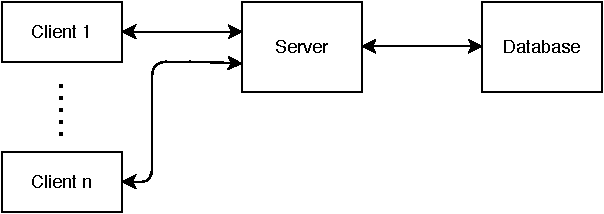
\includegraphics[scale=1]{img/traditional.pdf}
\caption{Traditional Design}
\label{trad}
\end{figure}

\subsection{Naive Design}
Someone might arrive at the nieve design shown in Figure \ref{naive} to crack
the problem of player interoperability. This will allow player to move from game
to game, however it's fondamentally flawed.

\begin{figure}[H]
\centering
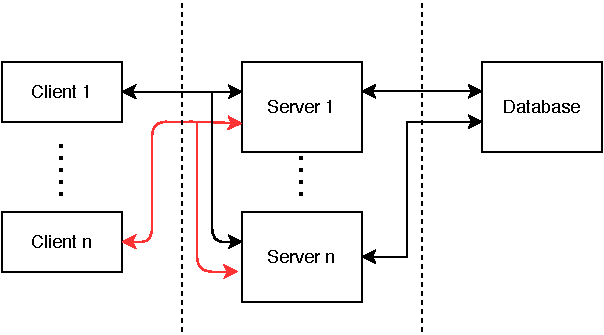
\includegraphics[scale=1]{img/nieve.pdf}
\caption{Naive Design}
\label{naive} 
\end{figure}

The issue being... servers with malicious intent have write capabilities on the
database, they can create unbounded wealth, distroy players assets, etc...

\subsection{Worlds Design}

\begin{figure}[H]
\centering
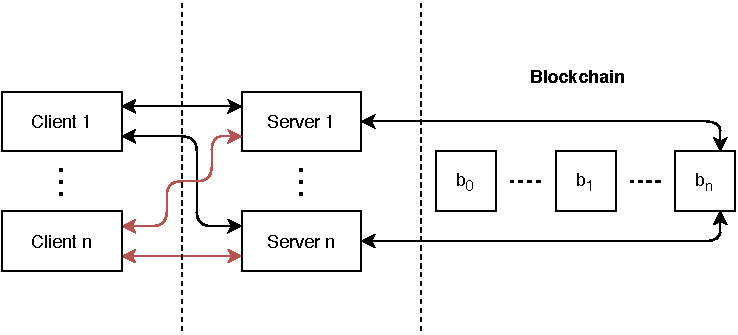
\includegraphics[scale=1]{img/worlds.pdf}
\caption{Worlds Design}
\label{fig:Worlds}
\end{figure}

A simplified version of the Worlds design is shown in Figure \ref{fig:Worlds}.
For more details please see the orrignal Worlds whitepaper. This is the ideal
and the nexus point where distributed games will be in the future, this will
allow player to place full control over their items to be clear - this is the
final goal.
\\

In the intereum, we need to build something a little bit easier for devleopers
to build with.

\subsubsection{Issues}

The problem is game developement is challanging, and adding the additional later to games
of querying a blockchain to understand the state of a game is simply too much to
ask for developers.

\section{Worlds.db}
We want the best aspect from both the
centralised and deventralised system.

\begin{enumerate}
\item Centralised databases enable simple integration.
\item Blockchain grants user driven control of assets, and player interteroperability.
\end{enumerate}


\begin{figure}[H]
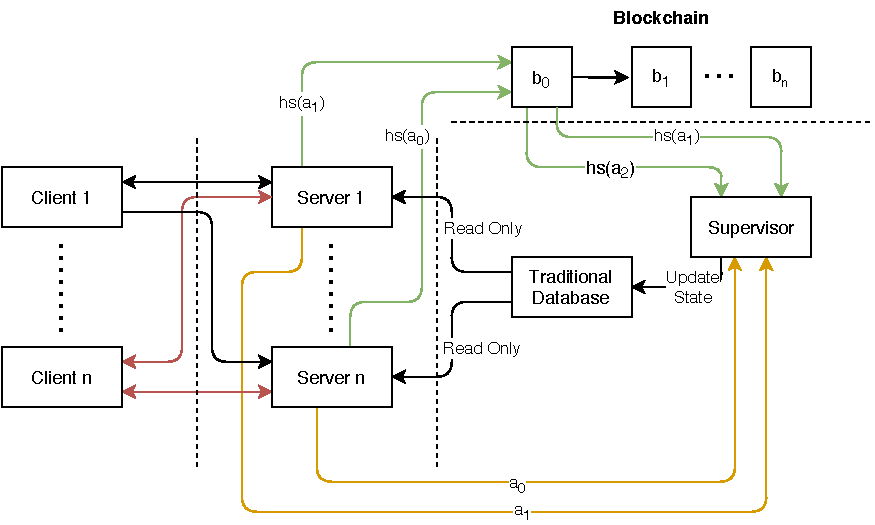
\includegraphics[]{img/worldsdb.pdf}
\caption{Worlds.db}
\label{fig:worldsdb}
\end{figure}

Figure \ref{fig:worldsdb} depicts the proposed structure. At a glance it looks
complicated. Howver the implementation is much simpler than Figure
\ref{fig:Worlds}. Lets outline the flow.

\begin{itemize}
\item The traditional database becomes read only from the servers perspective.
\item When servers want to update their game state they create $a$ - the database request.
\begin{itemize}
\item $a$ is just a string of the sql, mongo, etc... query.
\end{itemize}
\item $a$ sent to the supervisor (and broadcasted), the hash of $a$ .. $hs(a)$ is staked against and sent to the blockchain.
\begin{itemize}
\item The staked amount is a function of the database query itself.
\end{itemize}
\item The supervisor ensures $hs(a)$ is correct with $a$.
\item The supervisor update the state in the traditional database.
\end{itemize}

\subsection{Security}
It becomes obvious there are two centralised components of this structure. The
supervisor and the database. However this is recourse for a malicious attack. 
Since $a$ is broadcast, the comminity can reconstruct the state of the database though the
signed/submitted hashes to the blockchain. This allows for somewhat of a hard
fork away from the malcious database. 
\\

In addition you can incentivise the database maintainer to behave through a
monetary incentive.
\\

If further security is required, the database system can horizontally scale to
create redundant systems. This enables more robust error detection within
several databases.

\section{Advantages}
The biggest advantage of this structure is the simplicity of implementation on the
server side. Instead of modifying the code to quiery a blockchain directly
developers can continue to query a traditional database with the only modification
being instead of sending the mutable requests to the database, they are sent
directly to the supervisor. 

\section{Conclusion}
Time to build it.

\end{document}

